\documentclass[tikz,border=2pt]{standalone}
\usepackage{amsmath}
\usetikzlibrary{arrows.meta,calc,decorations.pathmorphing,positioning}

\definecolor{ink}{HTML}{263746}
\definecolor{muted}{HTML}{667785}
\definecolor{film}{HTML}{EAF1F3}
\definecolor{teal}{HTML}{2A8C82}
\definecolor{teallight}{HTML}{B9DDD7}
\definecolor{amber}{HTML}{D28A28}
\definecolor{amberlight}{HTML}{F5DFC0}

\begin{document}
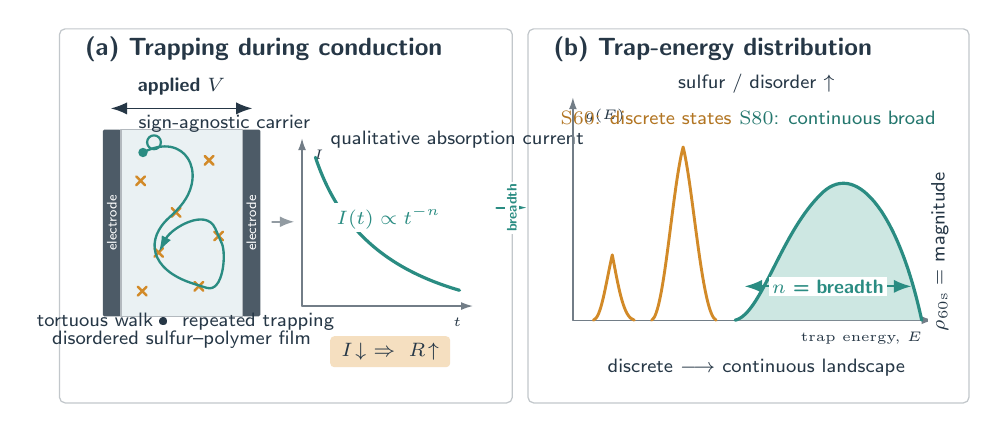
\begin{tikzpicture}[
  x=1cm,y=1cm,
  font=\sffamily,
  line cap=round,line join=round,
  >=Latex,
  panel/.style={draw=ink!28,rounded corners=2pt,line width=.45pt,fill=white},
  heading/.style={font=\sffamily\bfseries\small,text=ink,anchor=west},
  note/.style={font=\sffamily\scriptsize,text=muted,align=center},
  flow/.style={-{Latex[length=2.1mm,width=1.3mm]},line width=.85pt,draw=teal},
  trap/.style={draw=amber,line width=.9pt},
  axis/.style={-{Latex[length=1.5mm,width=1mm]},draw=ink!65,line width=.45pt}
]

% Two compact explanatory blocks
\draw[panel] (0,0) rectangle (5.75,4.75);
\draw[panel] (5.95,0) rectangle (11.55,4.75);
\node[heading] at (0.20,4.49) {(a) Trapping during conduction};
\node[heading] at (6.15,4.49) {(b) Trap-energy distribution};

% Panel A: biased cell and disordered, repeated trapping
\node[note,text=ink,font=\sffamily\scriptsize\bfseries] at (1.55,4.02) {applied $V$};
\draw[<->,draw=ink,line width=.65pt] (0.65,3.74) -- (2.45,3.74);
\draw[fill=ink!82,draw=none,rounded corners=.5pt] (0.55,1.10) rectangle (0.78,3.47);
\draw[fill=ink!82,draw=none,rounded corners=.5pt] (2.32,1.10) rectangle (2.55,3.47);
\draw[fill=film,draw=ink!35,line width=.45pt] (0.78,1.10) rectangle (2.32,3.47);
\node[rotate=90,font=\sffamily\tiny,text=white] at (0.665,2.285) {electrode};
\node[rotate=90,font=\sffamily\tiny,text=white] at (2.435,2.285) {electrode};
\node[note,text=ink] at (1.55,0.80) {disordered sulfur--polymer film};

% Unlabelled crosses denote illustrative trap sites only
\foreach \x/\y in {1.05/1.42,1.77/1.48,1.26/1.91,2.02/2.12,1.48/2.42,1.03/2.82,1.90/3.08}{
  \draw[trap] (\x-.055,\y-.055)--(\x+.055,\y+.055)
              (\x-.055,\y+.055)--(\x+.055,\y-.055);
}

% The meandering path avoids a clean ballistic-drift interpretation
\draw[flow,rounded corners=3pt]
  (1.06,3.18) .. controls (1.60,3.46) and (1.88,2.92) .. (1.48,2.43)
  .. controls (1.08,2.08) and (1.15,1.70) .. (1.77,1.49)
  .. controls (2.08,1.40) and (2.12,1.89) .. (2.02,2.12)
  .. controls (1.86,2.48) and (1.42,2.22) .. (1.26,1.91);
\fill[teal] (1.06,3.18) circle (1.7pt);
\draw[teal,line width=.8pt] (1.20,3.31) circle (2.5pt);
\node[note,anchor=west,align=left,text=ink] at (0.88,3.55) {sign-agnostic carrier};
\node[note,align=left,text=ink] at (1.60,1.03) {tortuous walk\;\textbullet\; repeated trapping};

% Qualitative current inset, visually separated from labels
\draw[axis] (3.08,1.23) -- (5.25,1.23) node[below left=1pt,font=\tiny,text=ink] {$t$};
\draw[axis] (3.08,1.23) -- (3.08,3.36) node[below right=1pt,font=\tiny,text=ink] {$I$};
\draw[draw=teal,line width=1.15pt]
  (3.25,3.12) .. controls (3.53,2.28) and (4.08,1.72) .. (5.08,1.43);
\node[note,text=ink,anchor=west,align=left] at (3.32,3.34)
  {qualitative absorption current};
\node[font=\sffamily\scriptsize\bfseries,text=teal,fill=white,inner sep=1.2pt]
  at (4.18,2.35) {$I(t)\propto t^{-n}$};
\node[note,text=ink,fill=amberlight,rounded corners=1.5pt,inner xsep=4pt,inner ysep=2.5pt]
  at (4.20,0.65) {$I\!\downarrow\ \Rightarrow\ R\!\uparrow$};
\draw[-{Latex[length=1.8mm]},draw=ink!50,line width=.55pt]
  (2.70,2.30) -- (2.98,2.30);

% Panel B: common axes, discrete low-S and broad high-S landscapes
\draw[axis] (6.52,1.05) -- (11.10,1.05) node[below left=1pt,font=\tiny,text=ink] {trap energy, $E$};
\draw[axis] (6.52,1.05) -- (6.52,3.88) node[below right=1pt,font=\tiny,text=ink] {$g(E)$};

% S60: separated narrow states (one dominant deep state)
\draw[draw=amber,line width=1.05pt]
  (6.78,1.05) .. controls (6.88,1.08) and (6.93,1.48) .. (7.02,1.88)
  .. controls (7.10,1.47) and (7.16,1.08) .. (7.30,1.05);
\draw[draw=amber,line width=1.05pt]
  (7.52,1.05) .. controls (7.68,1.12) and (7.78,2.72) .. (7.92,3.25)
  .. controls (8.05,2.72) and (8.16,1.12) .. (8.34,1.05);
\node[note,text=amber!85!black,align=left] at (7.45,3.62)
  {$\mathrm{S60}$: discrete states};

% S80: one continuous broad distribution
\path[fill=teallight!72,draw=none]
  (8.58,1.05) .. controls (8.92,1.13) and (9.16,2.18) .. (9.70,2.68)
  .. controls (10.15,3.08) and (10.67,2.35) .. (10.95,1.05) -- cycle;
\draw[draw=teal,line width=1.15pt]
  (8.58,1.05) .. controls (8.92,1.13) and (9.16,2.18) .. (9.70,2.68)
  .. controls (10.15,3.08) and (10.67,2.35) .. (10.95,1.05);
\node[note,text=teal!85!black,align=left] at (9.88,3.62)
  {$\mathrm{S80}$: continuous broad};

% Orthogonal encodings: horizontal breadth vs vertical magnitude
\draw[<->,draw=teal,line width=.75pt]
  (8.70,1.48) -- (10.82,1.48);
\node[font=\sffamily\scriptsize\bfseries,text=teal,fill=white,inner sep=1pt]
  at (9.76,1.48) {$n$ = breadth};
\draw[<->,draw=ink!72,line width=.7pt]
  (11.18,1.08) -- (11.18,2.76);
\node[font=\sffamily\scriptsize,text=ink,rotate=90,fill=white,inner sep=1pt]
  at (11.18,1.92) {$\rho_{60\mathrm{s}}$ = magnitude};

% Composition-driven evolution and concise cross-panel bridge
\draw[-{Latex[length=2mm,width=1.2mm]},draw=ink!65,line width=.65pt]
  (7.85,4.05) -- (9.85,4.05);
\node[note,text=ink,fill=white,inner sep=1pt] at (8.85,4.05)
  {sulfur / disorder $\uparrow$};
\node[note,text=ink,align=center] at (8.85,0.45)
  {discrete $\longrightarrow$ continuous landscape};

\draw[-{Latex[length=2mm,width=1.2mm]},draw=teal,line width=.8pt]
  (5.55,2.48) -- (5.94,2.48);
\node[font=\sffamily\tiny\bfseries,text=teal,fill=white,inner sep=.7pt,rotate=90]
  at (5.745,2.48) {breadth};

\end{tikzpicture}
\end{document}
